\subsection{Class Diagram}

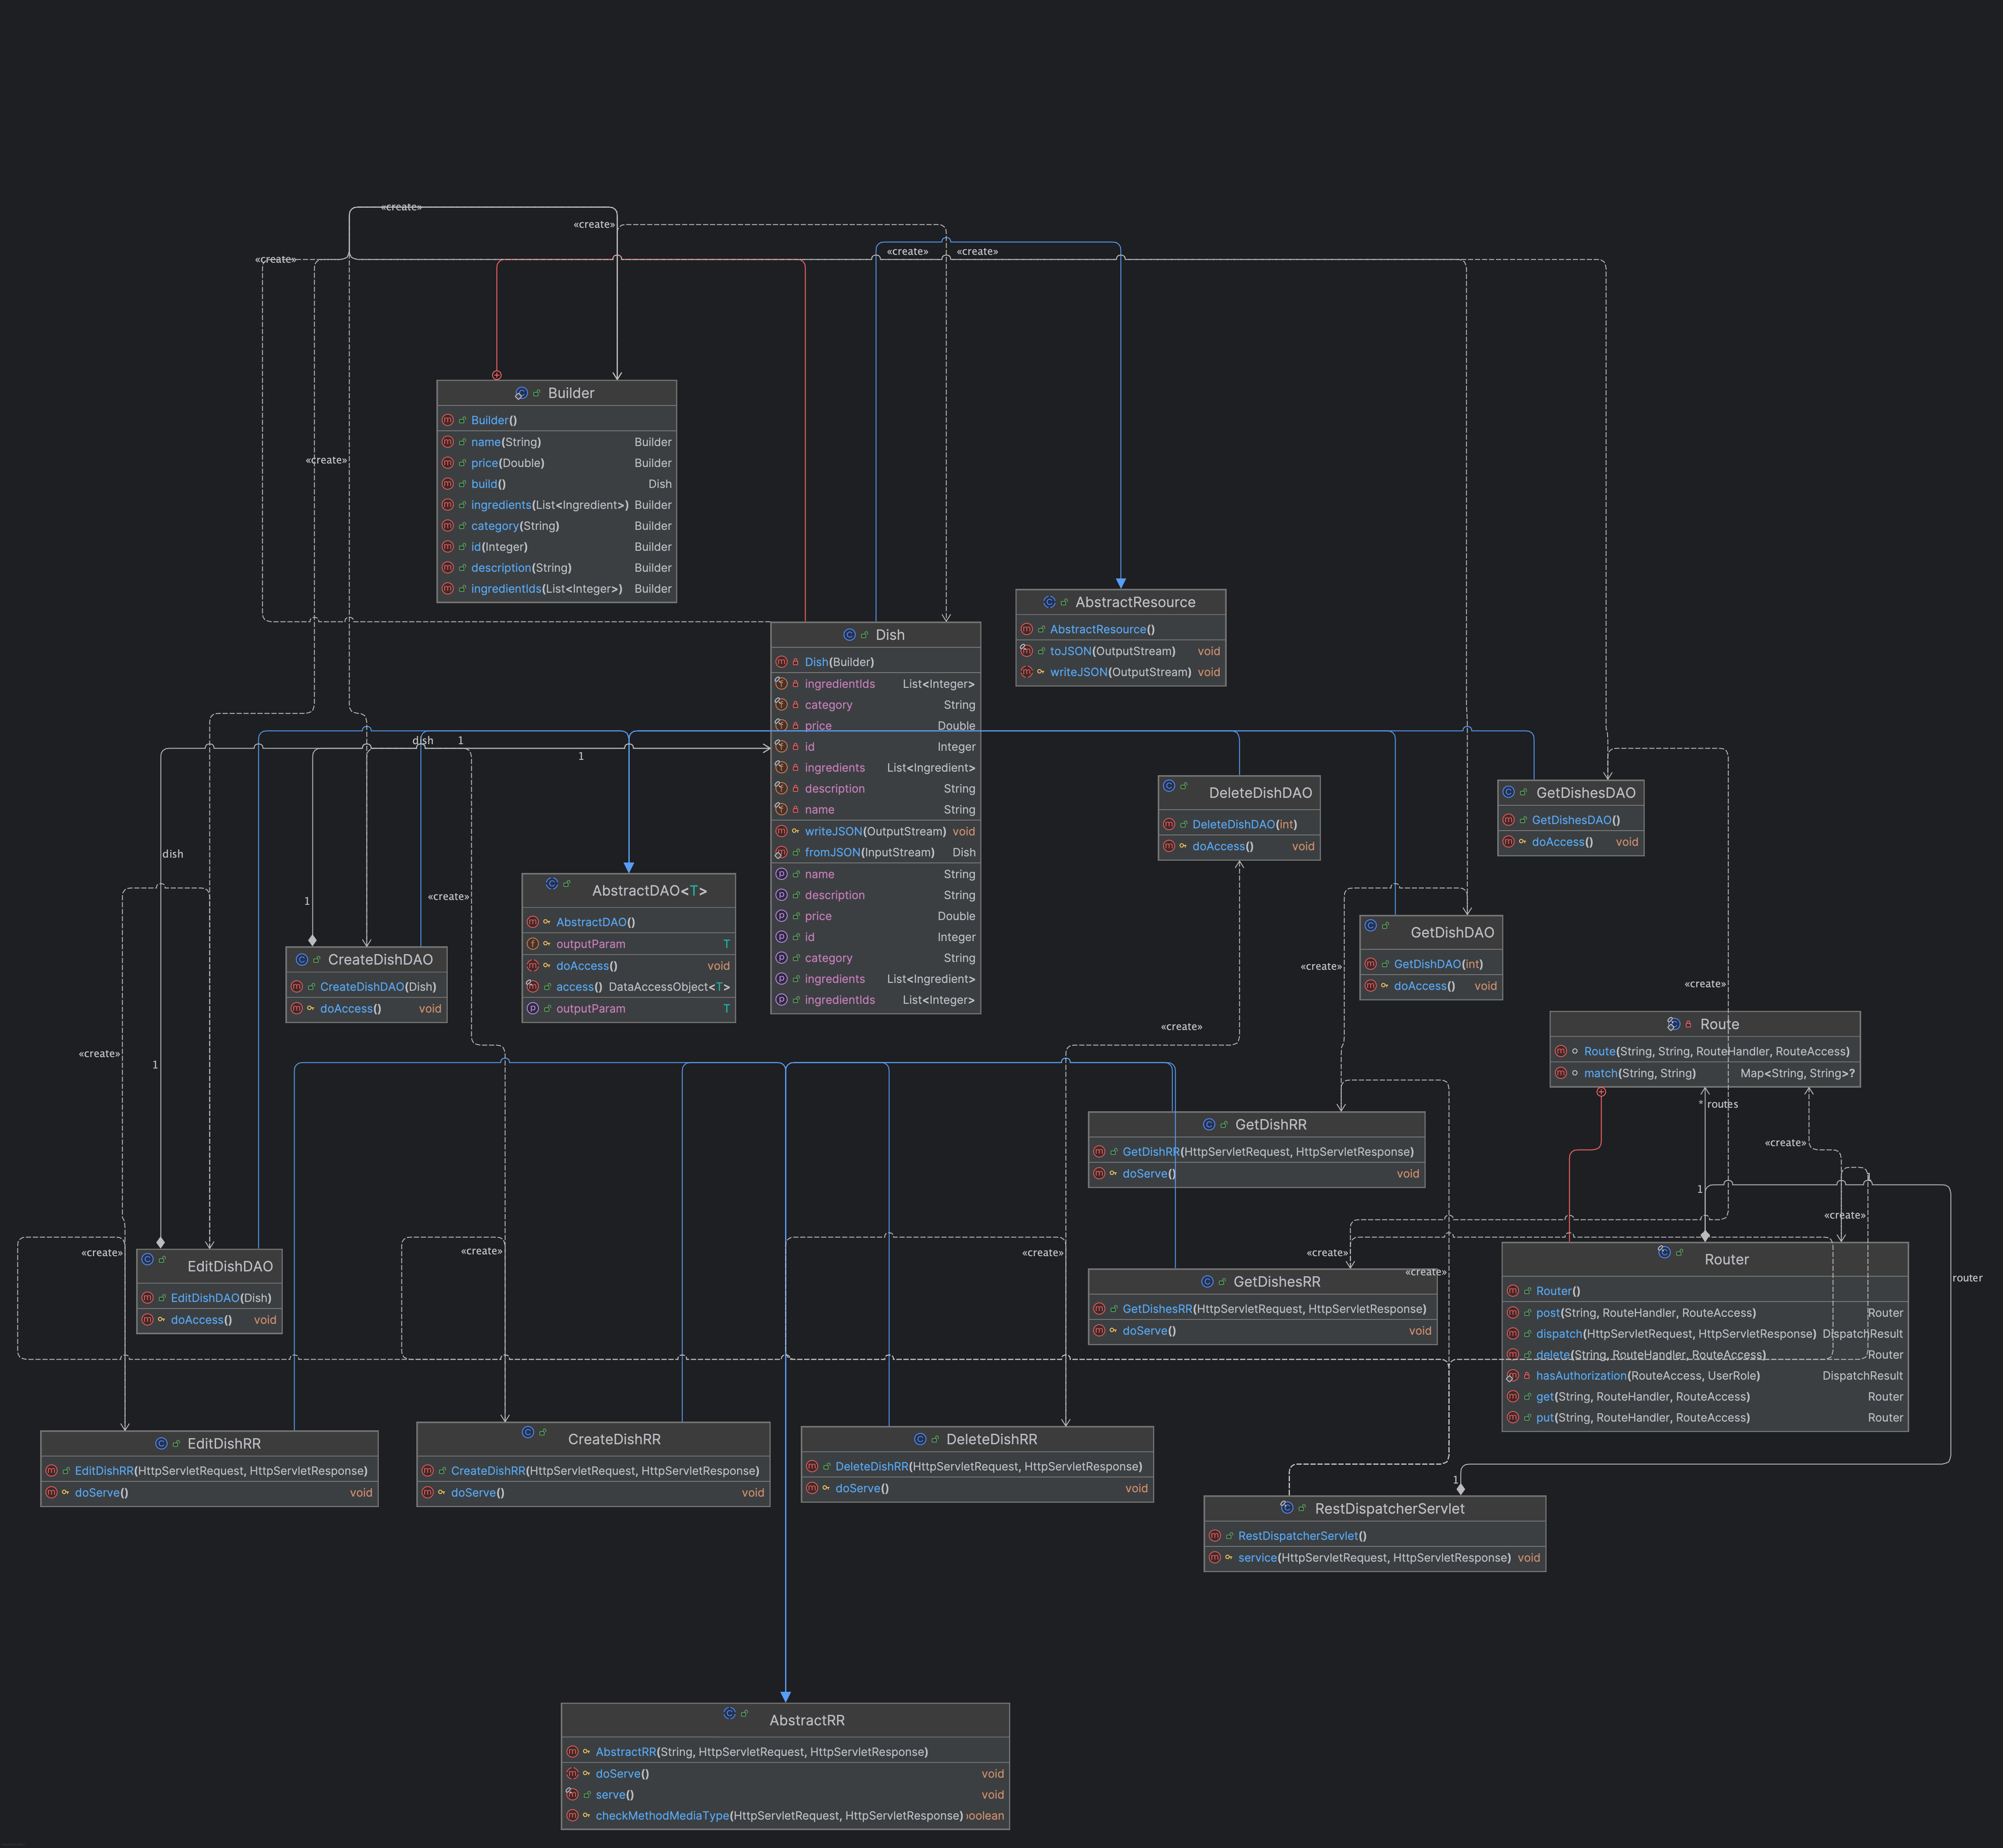
\includegraphics[width=\textwidth]{images/uml.png}

The business logic layer is organised into seven main packages:  \texttt{dao}, \texttt{exception}, \texttt{filter}, \texttt{resources}, \texttt{rest}, \texttt{servlet} and \texttt{util}.

\subsubsection*{resources}
Contains the classes that model the application data and are responsible for their own JSON serialisation. The root of the hierarchy is the \texttt{Resource} interface, which declares the single method \texttt{toJSON(OutputStream)}. \texttt{AbstractResource} provides a shared implementation backed by a Jackson \texttt{JsonFactory}, delegating the actual writing to the abstract method \texttt{writeJSON(OutputStream)}, which every concrete class must implement. The concrete resource classes are: \texttt{User} (uses the Builder pattern; password and hash are never serialised to JSON), \texttt{Credentials} (login payload, never serialised), \texttt{Item}, \texttt{Ingredient}, \texttt{Order}, \texttt{Promotion}, and \texttt{Message} (error/info wrapper with optional \texttt{error\_code} and \texttt{error\_details} fields). Supporting types include the enums \texttt{UserRole} (\texttt{STAFF}, \texttt{CUSTOMER}, \texttt{ADMIN}), \texttt{OrderStatus} (\texttt{PENDING}, \texttt{COMPLETED}, \texttt{CANCELLED}), \texttt{Allergen} (14 EU allergens), and \texttt{ItemCategory} (predefined menu categories with display name and description). \texttt{ResourceList<T>} serialises any collection of \texttt{Resource} objects as a JSON array.
 
\subsubsection*{rest}
Contains the per-endpoint controllers. \texttt{RestResource} is an interface declaring \texttt{serve()}. \texttt{AbstractRR} implements it and provides shared behaviour: MIME-type and HTTP method validation (checking \texttt{Accept} and \texttt{Content-Type} headers), structured error formatting via \texttt{Message} and per-thread logging via \texttt{LogContext}. Concrete subclasses override \texttt{doServe()}. Currently implemented: \texttt{RegisterUserRR} (handles \texttt{POST /rest/user/register}) and \texttt{AuthenticateUserRR} (handles \texttt{POST /rest/user/login}).
 
\subsubsection*{servlet}
Contains the front-controller infrastructure. \texttt{RestDispatcherServlet} is a \texttt{@WebServlet} mapped to \texttt{/rest/*}; it sets the client IP in \texttt{LogContext}, delegates routing to a \texttt{Router} instance and handles any uncaught \texttt{Throwable} by returning \texttt{500}. \texttt{Router} matches HTTP method and path against registered \texttt{Route} objects, supports path parameters (e.g.\ \texttt{/rest/user/\{id\}}) and stores extracted parameters as request attributes. \texttt{RouteHandler} is a \texttt{@FunctionalInterface} used as the handler type, allowing checked exceptions to propagate.
 
\subsubsection*{filter}
Contains the Jakarta Servlet filters applied to incoming HTTP requests. The package currently contains one class: \texttt{AuthFilter}, annotated with \texttt{@WebFilter(urlPatterns = "/dashboard/*")}. Its \texttt{doFilter()} method calls the private helper \texttt{extractTokenFromCookies()}, which iterates over the request cookies looking for the one whose name equals \texttt{JWTUtil.COOKIE\_NAME} (\texttt{auth\_token}). If no such cookie is found the method returns \texttt{null} and \texttt{doFilter()} immediately redirects to \texttt{/login}. If the cookie is found, \texttt{JWTUtil.verify(token)} is called. A \texttt{JWTVerificationException} (that means invalid signature or expired token) causes a redirect to \texttt{/login}. On successful verification the \texttt{user\_id} claim is extracted from the \texttt{DecodedJWT} and stored as a request attribute. Then \texttt{chain.doFilter()} passes control to the next component in the pipeline.
 
\subsubsection*{dao}
Contains the Data Access Objects. \texttt{DataAccessObject<T>} is an interface that declares \texttt{access()} and \texttt{getOutputParam()}. \texttt{AbstractDAO<T>} implements this interface and manages the full connection lifecycle. The latter acquires a connection from \texttt{ConnectionPoolSingleton} at construction time, calls \texttt{doAccess()} inside a try/catch block, commits or rolls back as needed and closes the connection. It also prevents double-calling via a \texttt{synchronized} accessed flag.
 
The concrete DAOs are organised in sub-packages by domain:
\begin{itemize}
    \item \textbf{Root package}: \texttt{RegisterUserDAO} (inserts a new user with bcrypt hash, returns the generated \texttt{id}); \texttt{AuthenticateUserDAO} (looks up user by email, verifies password with bcrypt, returns \texttt{user\_id} or \texttt{null}).
    \item \textbf{ingredient}: \texttt{NewIngredientDAO} (inserts an ingredient, converts allergen list to a SQL array); \texttt{GetIngredientDAO} (selects a single ingredient by id, deserialises the SQL allergen array); \texttt{GetIngredientsDAO} (selects all ingredients ordered by id); \texttt{EditIngredientDAO} (updates name, is\_frozen, and allergen of an existing ingredient); \texttt{DeleteIngredientDAO} (deletes an ingredient by id, returns \texttt{Boolean} success flag).
    \item \textbf{item}: \texttt{CreateItemDAO} (inserts an item after validating non-null name, description, non-negative price, and non-null ingredients); \texttt{DeleteItemDAO} (deletes an item by id); \texttt{BindIngredientDAO} (inserts rows into \texttt{item\_ingredients} for all ingredients of an item); \texttt{BindCategoryDAO} (inserts rows into \texttt{item\_categories} for all categories of an item, validating that each \texttt{ItemCategory} has a non-empty name and description).
    \item \textbf{order}: \texttt{NewOrderDAO} (inserts an order, rejects null order or negative total price via a \texttt{NotValidOrder} runtime exception in the constructor); \texttt{GetOrderDAO} (retrieves a single order by id); \texttt{GetOrdersDAO} (retrieves all orders); \texttt{EditOrderDAO} (updates the status of an order); \texttt{DeleteOrderDAO} (deletes an order by id).
    \item \textbf{promotions}: \texttt{NewPromotionDAO} (inserts a promotion after validating it is not null and not expired); \texttt{CheckPromotionDAO} (looks up a promotion by code, throws \texttt{NotValidPromotionException} if not found or expired).
\end{itemize}
 
\subsubsection{exception}
Contains domain-specific checked exceptions used to signal validation failures at construction time or during DAO access: \texttt{MalformedJSONException} (malformed JSON request body, with multiple constructors), \texttt{NotValidIngredientException}, \texttt{NotValidItemException}, \texttt{NotValidCategoryException}, \texttt{NotValidPromotionException}, \texttt{ServiceException}. \texttt{NotValidOrder} is instead an unchecked \texttt{RuntimeException}, thrown in the \texttt{NewOrderDAO} constructor.
 
\subsubsection{util}
Contains cross-cutting utilities. \texttt{JWTUtil} is a static helper that initialises an HMAC-256 signer from the \texttt{jwt.secret} context parameter (read at startup by \texttt{AppContextListener}) and exposes \texttt{generateToken(int userId)} and \texttt{verify(String token)}; tokens contain the \texttt{user\_id} claim and expire in 8 hours (28800 seconds). \texttt{Validator} provides static methods \texttt{isValidEmail} and \texttt{isValidPassword} using compiled regex patterns. \texttt{ConnectionPoolSingleton} looks up and exposes the container-managed JNDI \texttt{DataSource}. \texttt{AppContextListener} implements \texttt{ServletContextListener} and calls \texttt{JWTUtil.init()} at application startup. \texttt{ErrorCodes} centralises all error code string constants. \texttt{LogContext} wraps Log4j2's \texttt{ThreadContext} to store per-request context (IP address, action, resource) for structured logging. \texttt{Actions} holds string constants for the action names used in logging.
 
\subsubsection{test}
The project includes a unit test class \texttt{JWTUtilTest}, which verifies that a generated token contains the expected \texttt{user\_id} claim, that a token signed with a different secret is rejected, and that a malformed string is rejected by \texttt{JWTUtil.verify()}.